\documentclass{article}
\usepackage[utf8]{inputenc}
\usepackage{typearea}
\usepackage{multirow}
\usepackage{color, colortbl}
\usepackage{caption}
\usepackage{subcaption}
\usepackage{graphicx}
\usepackage{float}
\definecolor{Gray}{RGB}{231, 230, 230}

\title{Exercício 1 - Métodos Diretos e Métodos Iterativos Estacionários}
\author{Lorena B. Bassani$^1$}
\date{2021}

\begin{document}

\maketitle

\begin{abstract}
    Este documento relata os resultados do primeiro exercício da disciplina de Algoritmos Numéricos II, no semestre 2021/01 EARTE. Seu objetivo é Observar o comportamento dos Métodos diretos e iterativos estacionários quanto as características da matriz dos coeficientes.
\end{abstract}

\section{Introdução}
Para este exercício, foram utilizadas cinco matrizes esparsas, duas de dimensão $100\times100$, uma de dimensão $289\times289$, uma de dimensão $1000\times1000$ e uma de dimensão $1138\times1138$, obtidas da coleção de matrizes esparsas \textit{SuiteSparse Matrix Collection}. Nessas quatro matrizes, foram realizadas análises quanto ao comportamento de métodos diretos e iterativos estacionários, utilizando a ferramenta Octave e códigos fornecidos como material da disciplina. Na seção~\ref{sec:diretos} são relatadas algumas observações sobre a utilização de métodos diretos para resolução de sistemas lineares, enquanto na seção~\ref{sec:iterativos} é possível observar sobre os métodos iterativos estacionários. Na última parte do trabalho, na seção~\ref{sec:tabelas}, se encontram as tabelas com os resultados obtidos.

\section{Primeiro Exercício Proposto -- Métodos Diretos}
\label{sec:diretos}
O objetivo deste exercício é observar o comportamento de matrizes esparsas na solução de sistemas lineares via métodos diretos. Para isto, as matrizes escolhidas foram submetidas a decomposição LU através de método nativo do Octave, e foram observados uma série de fatores quanto ao comportamento das matrizes a respeito do preenchimento no processo de decomposição e seu condicionamento.

Na Tabela~\ref{tab:diretos}: Tabela de resultados observados em resolução de matrizes por métodos diretos, é possível observar alguns dos resultados obtidos através da resolução dos sistemas por Eliminação de Gauss.

Nas duas matrizes com $n=100$ a solução encontrada ficou bem próxima da solução exata, com distância relativa entre elas sendo bem pequena. A taxa de preenchimento foi relativamente alta na \textit{nos4} se comparado a \textit{tub100}, acarretando em mais espaço utilizado que com os métodos iterativos, enquanto a \textit{mesh3e1} de tamanho $n=289$ teve uma taxa muito alta de preenchimento, acima de 90\%.

Nas matrizes com dimensão igual ou superior a $n=1000$, as soluções ficaram mais distantes da solução exata, sendo que a \textit{sherman1} não parece ter respondido bem ao método de Eliminação de Gauss. A taxa de preenchimento de ambas foi muito alto, acima de 90\%, com um grande desperdício de espaço para armazenamento depois da fatoração LU. Nas figuras a seguir, é possível observar o preenchimento da Matriz original, assim como o das matrizes L e U da fatoração.

De todas as matrizes testadas, apenas a \textit{mesh3e1} parece ter um número de condicionamento menor, abaixo de 10, sendo a que tem a maior chance de ser bem condicionada dentre todas. A que apresentou o maior número foi a \textit{1138\_bus}, sendo provavelmente mal condicionada.

\begin{figure}[H]
    \centering
    \begin{subfigure}[b]{0.3\textwidth}
         \centering
         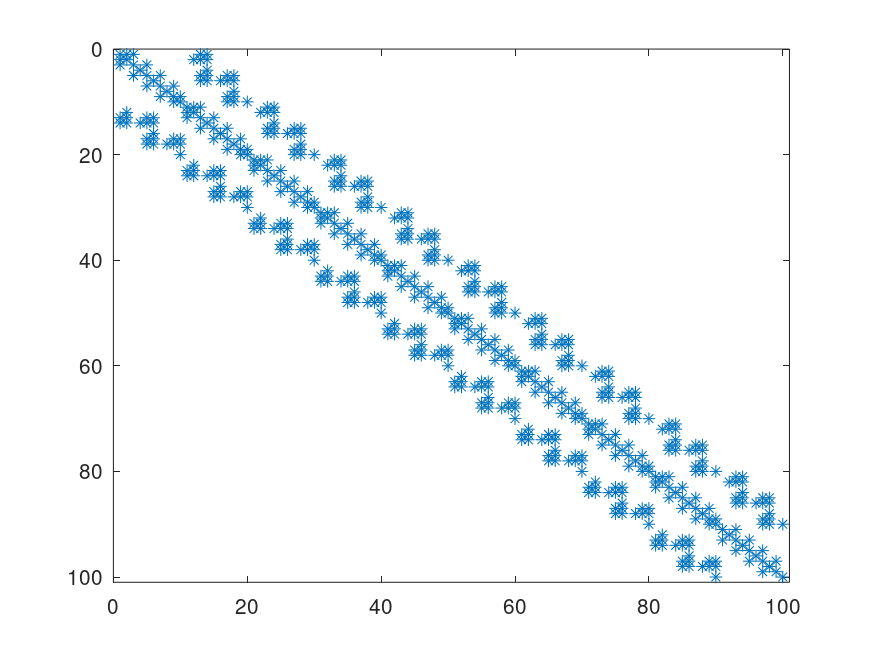
\includegraphics[width=\textwidth]{image/nos4spyA.png}
         \caption{Preenchimento de A}
         \label{fig:nos4-spyA}
    \end{subfigure}
    \hfill
    \begin{subfigure}[b]{0.3\textwidth}
         \centering
         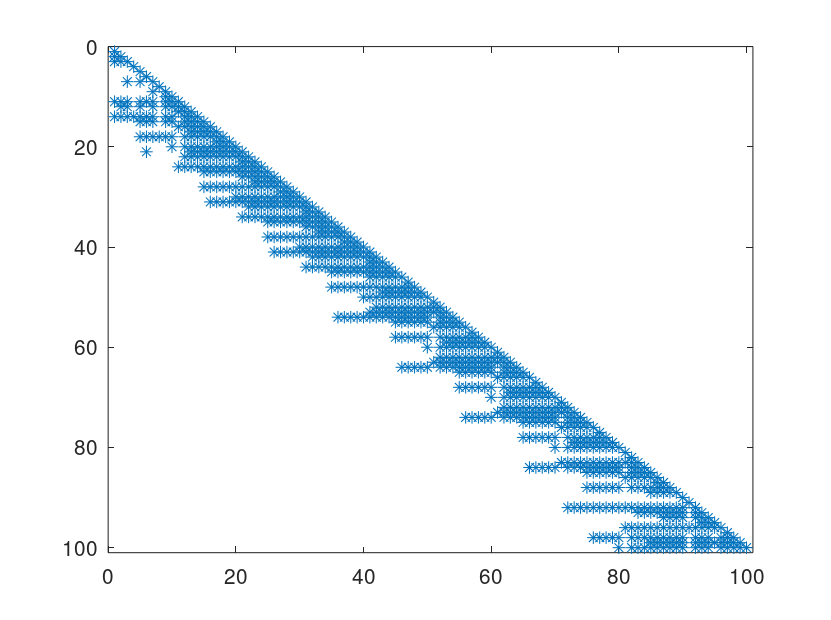
\includegraphics[width=\textwidth]{image/nos4spyL.png}
         \caption{Preenchimento de L}
         \label{fig:nos4-spyL}
    \end{subfigure}
    \hfill
    \begin{subfigure}[b]{0.3\textwidth}
         \centering
         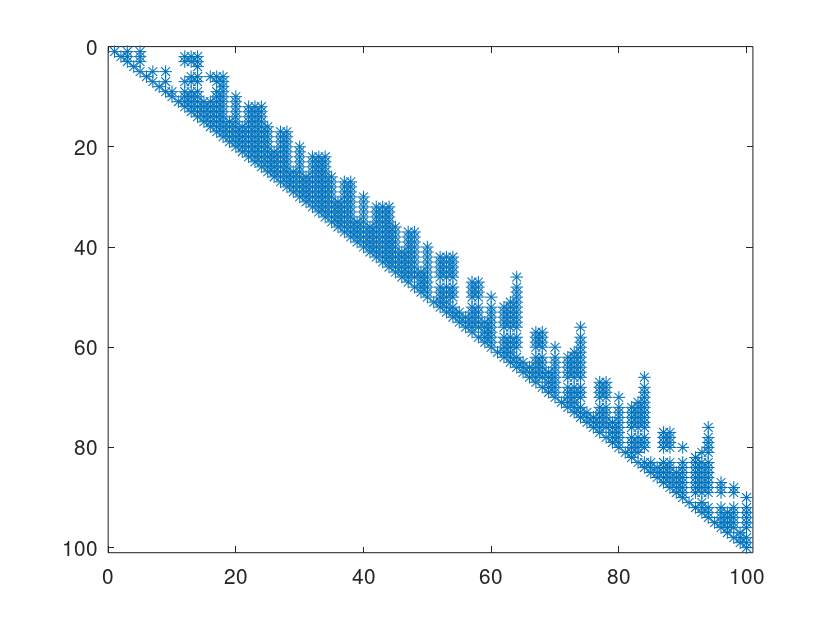
\includegraphics[width=\textwidth]{image/nos4spyU.png}
         \caption{Preenchimento de U}
         \label{fig:nos4-spyU}
    \end{subfigure}
    \hfill
    \caption{configuração de esparsidade das matrizes do sistema \textit{nos4}.}
    \label{fig:nos4}
\end{figure}

\begin{figure}[H]
    \centering
    \begin{subfigure}[b]{0.3\textwidth}
         \centering
         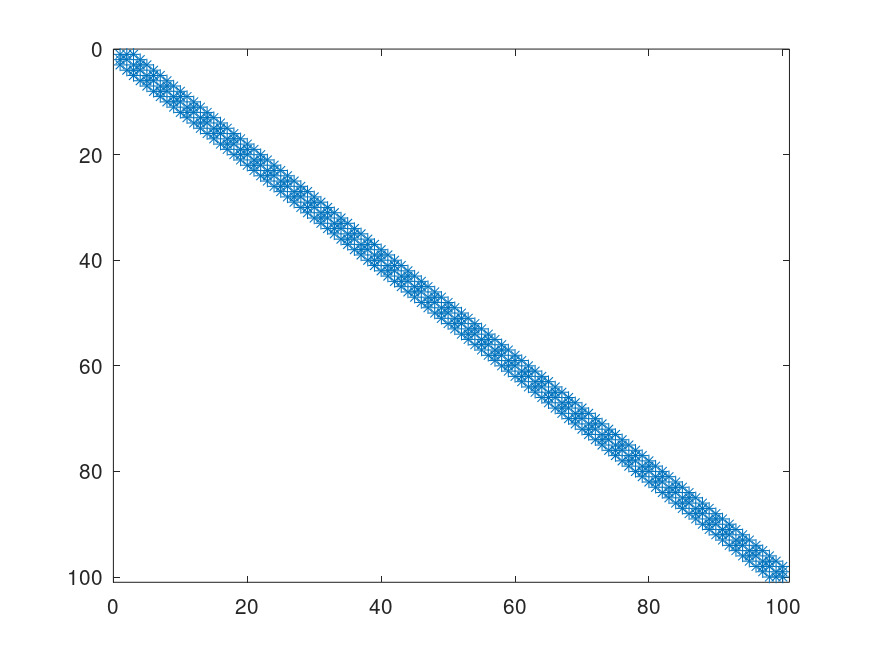
\includegraphics[width=\textwidth]{image/tub100spyA.png}
         \caption{Preenchimento de A}
         \label{fig:tub100-spyA}
    \end{subfigure}
    \hfill
    \begin{subfigure}[b]{0.3\textwidth}
         \centering
         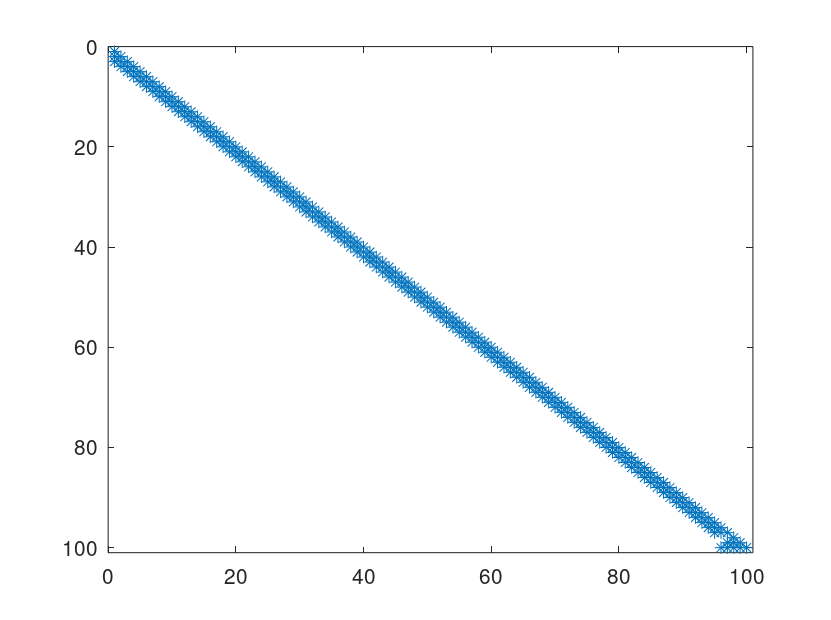
\includegraphics[width=\textwidth]{image/tub100spyL.png}
         \caption{Preenchimento de L}
         \label{fig:tub100-spyL}
    \end{subfigure}
    \hfill
    \begin{subfigure}[b]{0.3\textwidth}
         \centering
         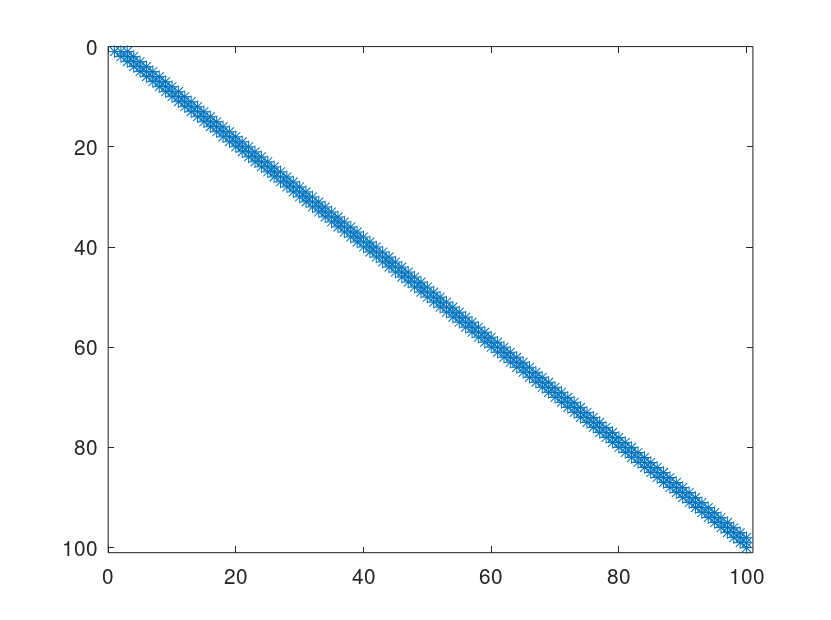
\includegraphics[width=\textwidth]{image/tub100spyU.png}
         \caption{Preenchimento de U}
         \label{fig:tub100-spyU}
    \end{subfigure}
    \hfill
    \caption{configuração de esparsidade das matrizes do sistema \textit{tub100}.}
    \label{fig:tub100}
\end{figure}

\begin{figure}[H]
    \centering
    \begin{subfigure}[b]{0.3\textwidth}
         \centering
         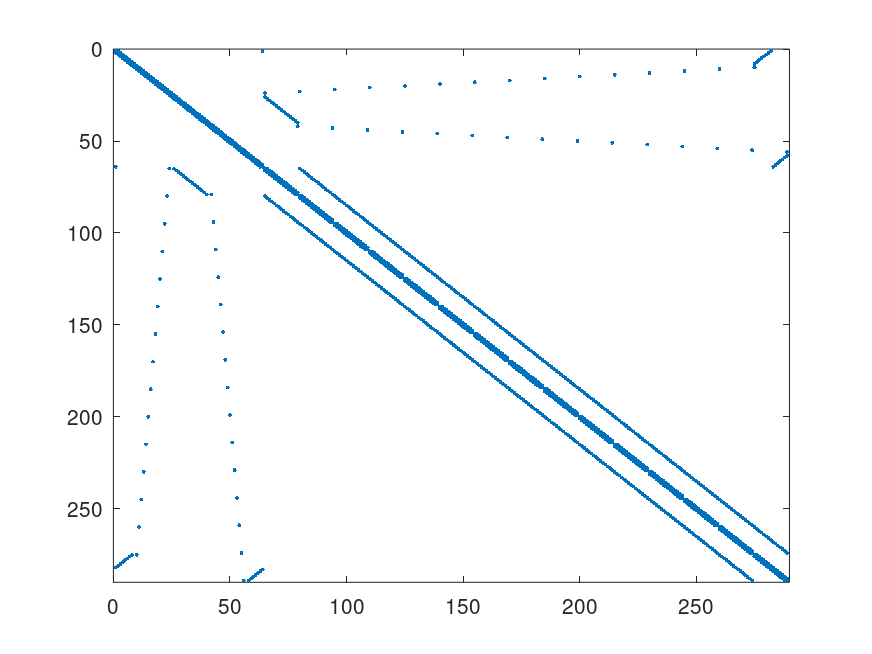
\includegraphics[width=\textwidth]{image/mesh3e1_spyA.png}
         \caption{Preenchimento de A}
         \label{fig:mesh-spyA}
    \end{subfigure}
    \hfill
    \begin{subfigure}[b]{0.3\textwidth}
         \centering
         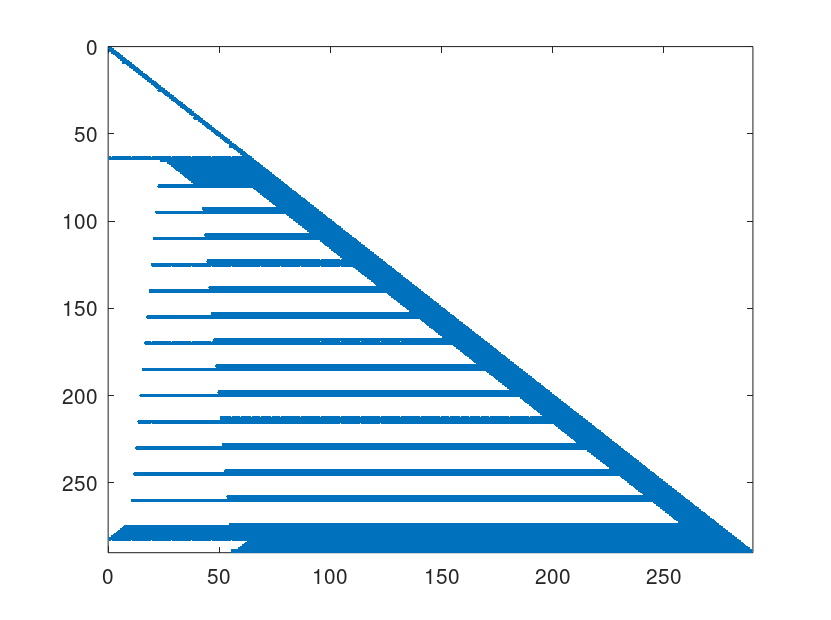
\includegraphics[width=\textwidth]{image/mesh3e1_spyL.png}
         \caption{Preenchimento de L}
         \label{fig:mesh-spyL}
    \end{subfigure}
    \hfill
    \begin{subfigure}[b]{0.3\textwidth}
         \centering
         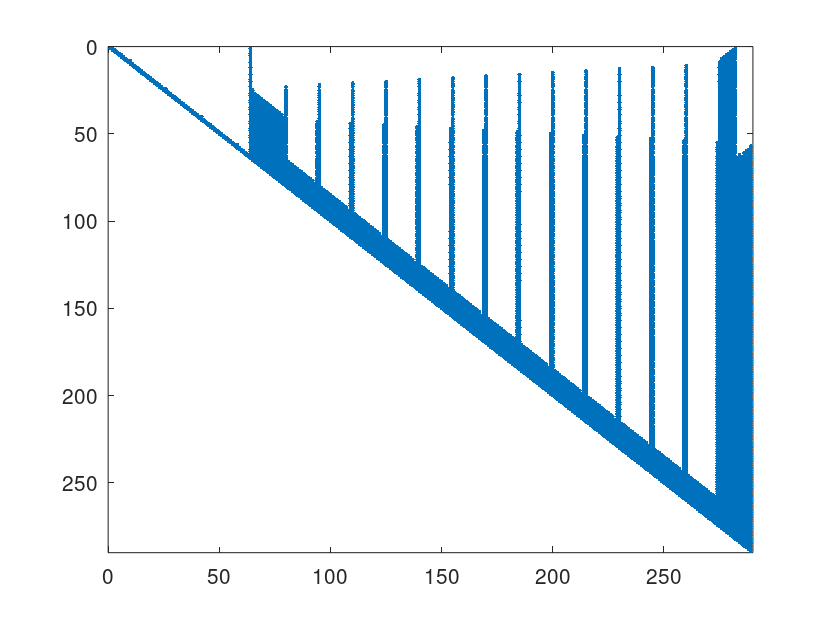
\includegraphics[width=\textwidth]{image/mesh3e1_spyU.png}
         \caption{Preenchimento de U}
         \label{fig:mesh-spyU}
    \end{subfigure}
    \hfill
    \caption{configuração de esparsidade das matrizes do sistema \textit{mesh3e1}.}
    \label{fig:mesh}
\end{figure}

\begin{figure}[H]
    \centering
    \begin{subfigure}[b]{0.3\textwidth}
         \centering
         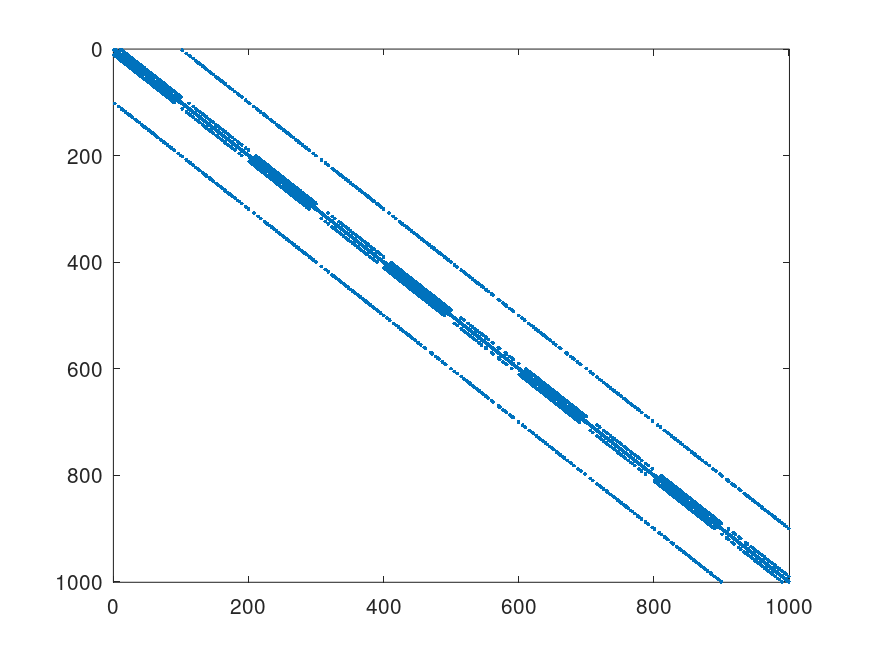
\includegraphics[width=\textwidth]{image/sherman1spyA.png}
         \caption{Preenchimento de A}
         \label{fig:sherman1-spyA}
    \end{subfigure}
    \hfill
    \begin{subfigure}[b]{0.3\textwidth}
         \centering
         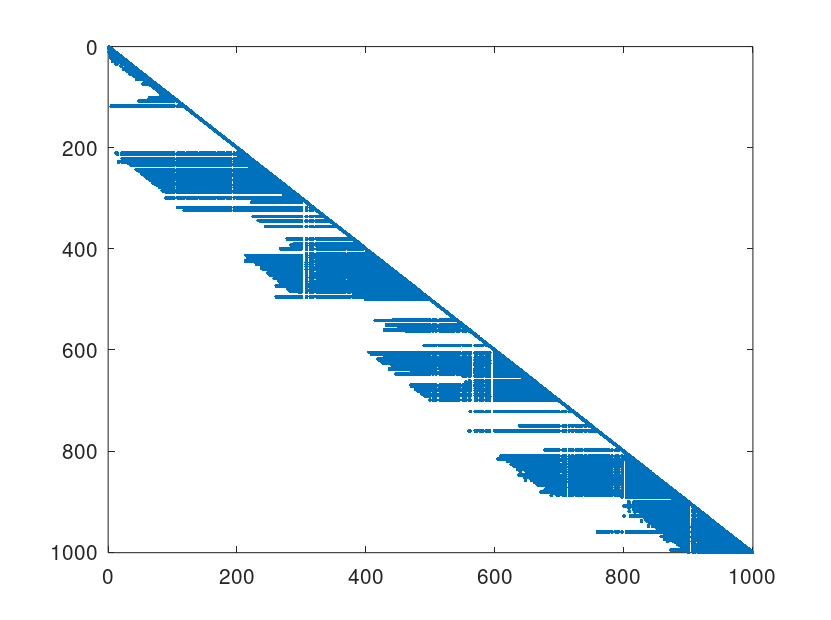
\includegraphics[width=\textwidth]{image/sherman1spyL.png}
         \caption{Preenchimento de L}
         \label{fig:sherman1-spyL}
    \end{subfigure}
    \hfill
    \begin{subfigure}[b]{0.3\textwidth}
         \centering
         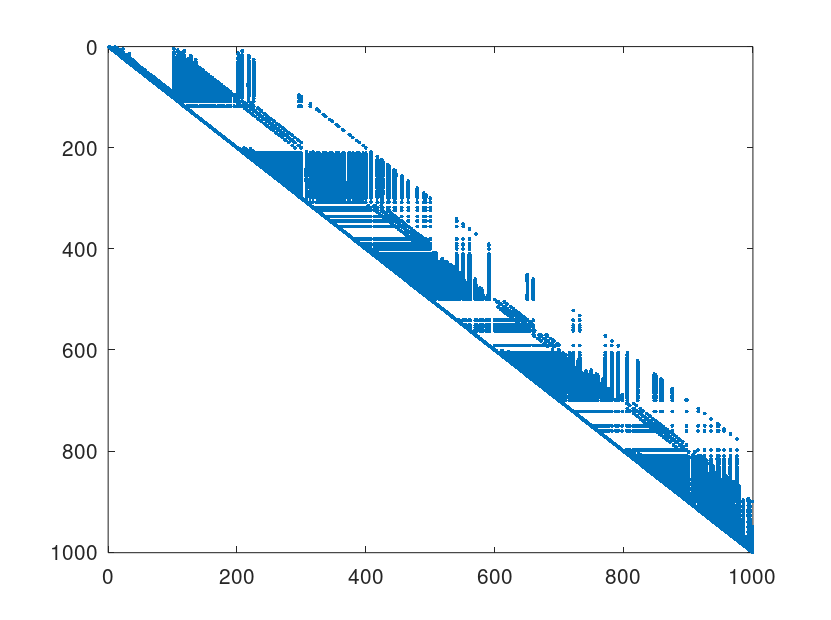
\includegraphics[width=\textwidth]{image/sherman1spyU.png}
         \caption{Preenchimento de U}
         \label{fig:sherman1-spyU}
    \end{subfigure}
    \hfill
    \caption{configuração de esparsidade das matrizes do sistema \textit{sherman1}.}
    \label{fig:sherman1}
\end{figure}

\begin{figure}[H]
    \centering
    \begin{subfigure}[b]{0.3\textwidth}
         \centering
         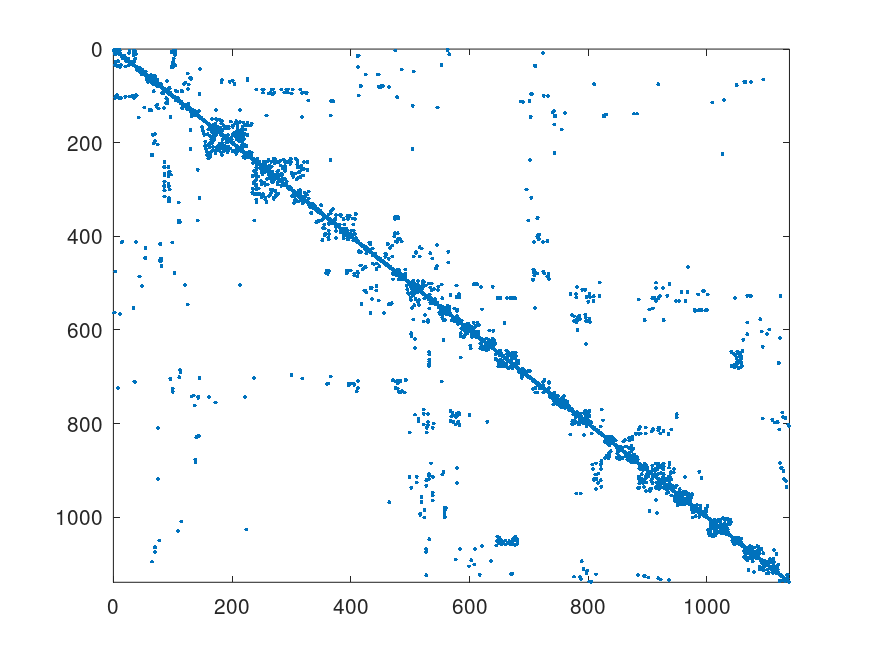
\includegraphics[width=\textwidth]{image/1138_bus_spyA.png}
         \caption{Preenchimento de A}
         \label{fig:bus-spyA}
    \end{subfigure}
    \hfill
    \begin{subfigure}[b]{0.3\textwidth}
         \centering
         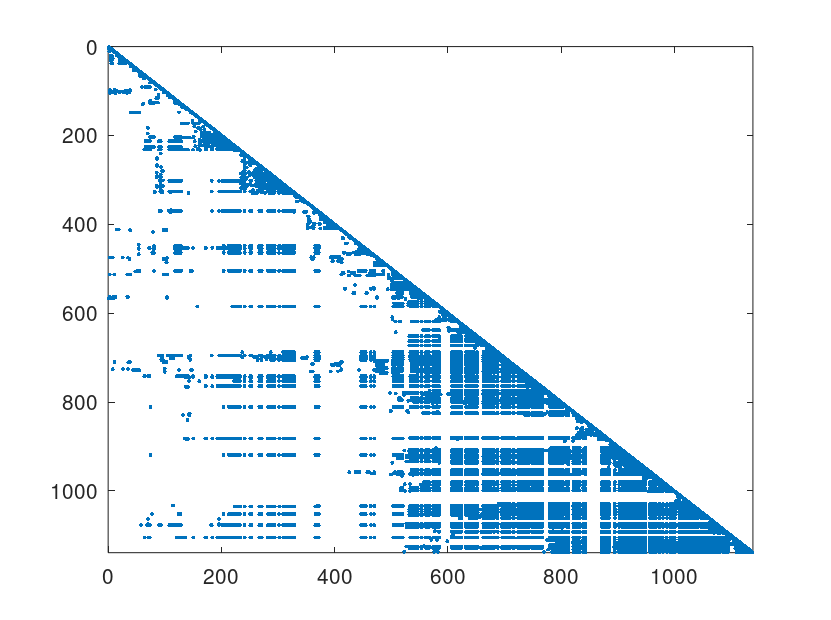
\includegraphics[width=\textwidth]{image/1138_bus_spyL.png}
         \caption{Preenchimento de L}
         \label{fig:bus-spyL}
    \end{subfigure}
    \hfill
    \begin{subfigure}[b]{0.3\textwidth}
         \centering
         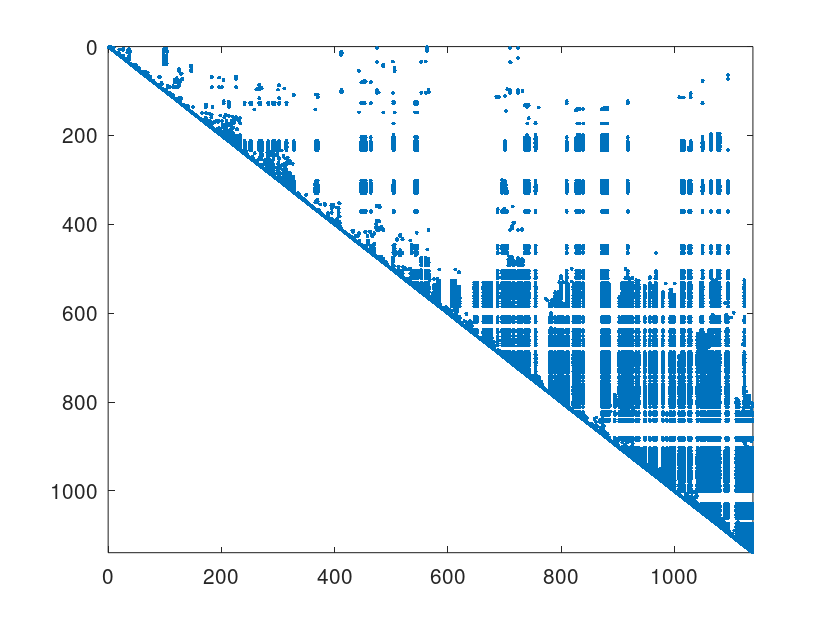
\includegraphics[width=\textwidth]{image/1138_bus_spyU.png}
         \caption{Preenchimento de U}
         \label{fig:bus-spyU}
    \end{subfigure}
    \hfill
    \caption{configuração de esparsidade das matrizes do sistema \textit{1138\_bus}.}
    \label{fig:bus}
\end{figure}

\section{Segundo Exercício Proposto -- Métodos Iterativos Estacionários}
\label{sec:iterativos}
O objetivo deste exercício é observar o comportamento de matrizes esparsas na solução de sistemas lineares via métodos iterativos estacionários. Foram utilizadas funções fornecidas como material da disciplina para resolução dos sistemas através dos métodos de Jacobi, Seidel e SOR.

Os algoritmos foram rodados com limite máximo de 1000 iterações e tolerância de 10$^{-3}$. Para encontrar o valor de w para o método SOR, foram rodados testes com 20 valores entre 2 e 0.1 nas matrizes de tamanho $n=100$, e 5 valores entre 2 e 1 nas matrizes de tamanho $n=1000$.

Na Tabela~\ref{tab:iterativos}: Tabela de resultados observados em resolução de matrizes por métodos iterativos estacionários, é possível observar alguns dos resultados obtidos através da resolução dos sistemas pelos métodos de Jacobi, Seidel e SOR.

Nas figuras a seguir é possível ver os gráficos que mostram a convergência dos métodos em relação a quantidade de iterações que foram necessárias para diminuir o erro da solução. 

\begin{figure}[H]
    \centering
    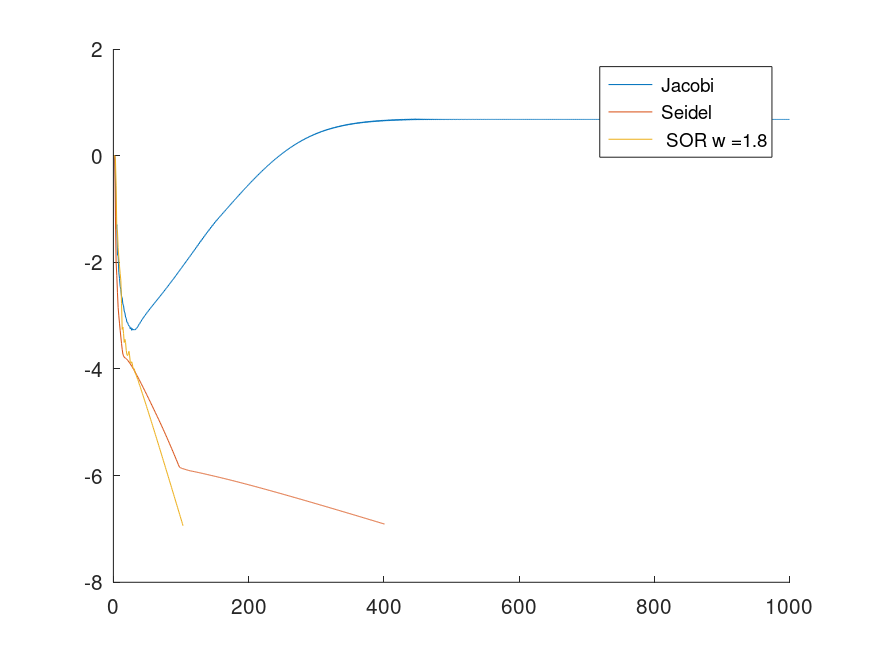
\includegraphics[width=.8\textwidth]{image/nos4iterativo.png}
    \caption{Gráfico de convergência do sistema \textit{nos4}}
    \label{fig:nos4-iter}
\end{figure}

\begin{figure}[H]
    \centering
    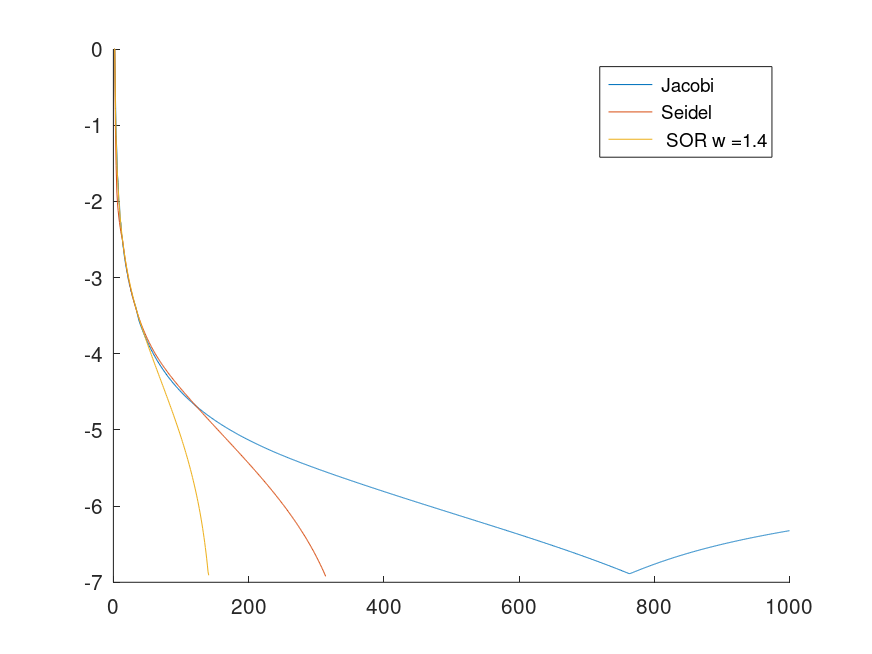
\includegraphics[width=.8\textwidth]{image/tub100iterativo.png}
    \caption{Gráfico de convergência do sistema \textit{tub100}}
    \label{fig:tub100-iter}
\end{figure}

\begin{figure}[H]
    \centering
    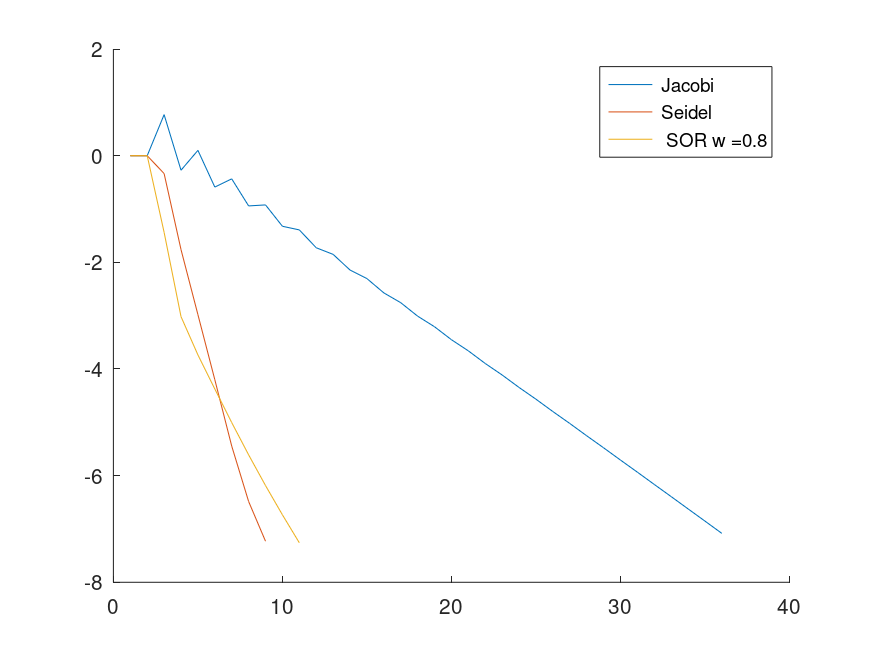
\includegraphics[width=.8\textwidth]{image/mesh3e1_iterativo.png}
    \caption{Gráfico de convergência do sistema \textit{mesh3e1}}
    \label{fig:mesh-iter}
\end{figure}

\begin{figure}[H]
    \centering
    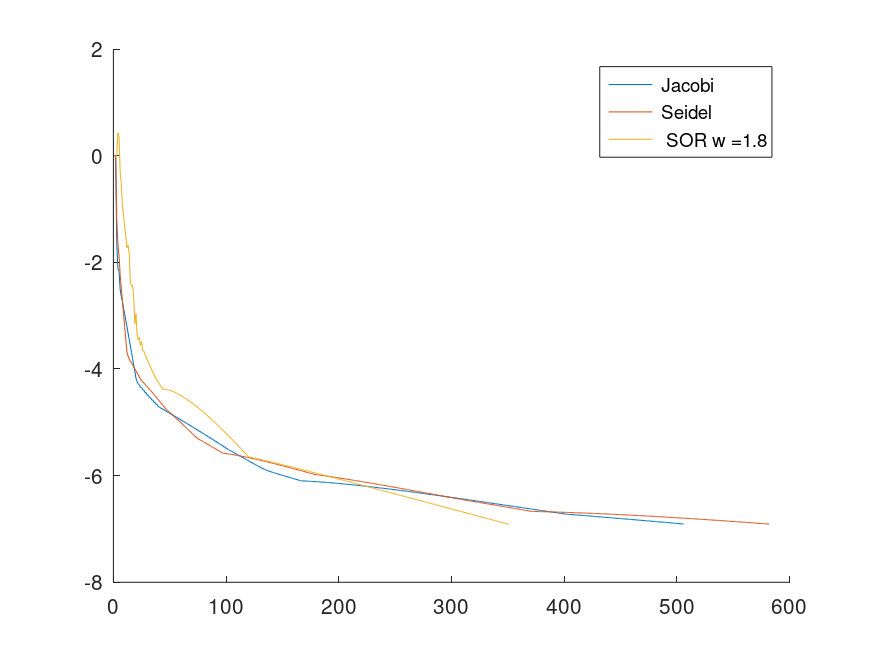
\includegraphics[width=.8\textwidth]{image/sherman1iterativo.png}
    \caption{Gráfico de convergência do sistema \textit{sherman1}}
    \label{fig:sherman1-iter}
\end{figure}

\begin{figure}[H]
    \centering
    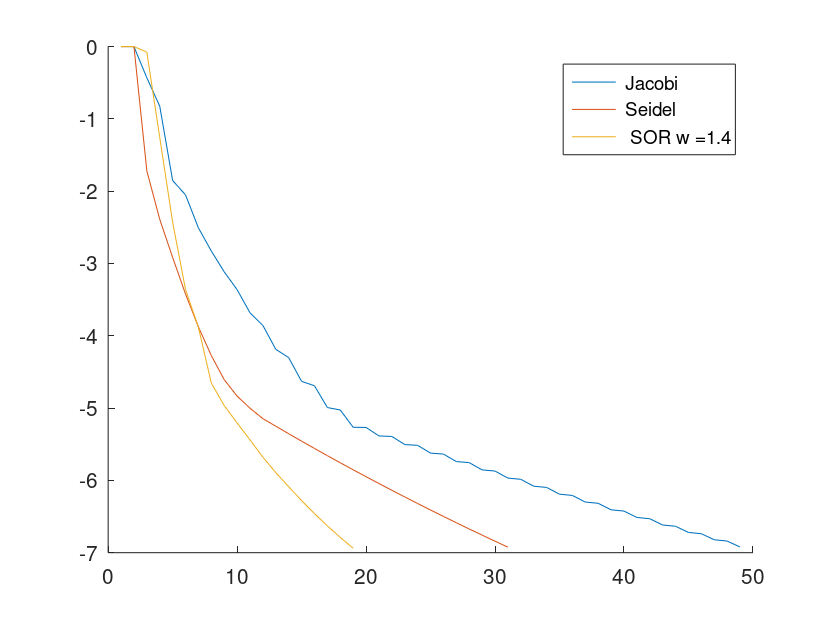
\includegraphics[width=.8\textwidth]{image/1138_bus_iterativo.png}
    \caption{Gráfico de convergência do sistema \textit{1138\_bus}}
    \label{fig:bus-iter}
\end{figure}
\newpage

Apenas uma das matrizes escolhidas--a \textit{mesh3e1}--era diagonal dominante, e nenhuma das duas de tamanho $n=100$ conseguiram convergir antes das 1000 iterações com método de Jacobi. Todas as matrizes tiveram convergência com os métodos SOR e Seidel, com o SOR atingindo o critério de parada de tolerância do erro relativo com menor número de iterações, menos para a matriz \textit{mesh3e1}, para o qual os valores de w testados não conseguiram melhorar em comparação ao método de Seidel. Apesar disso, o comportamento das que não convergiram para Jacobi mostra que, dependendo da tolerância, as matrizes que não são diagonal dominante podem chegar ao ponto de começar a aumentar o erro ao invés de diminuir. 

Na matriz \textit{nos4}, o método de Jacobi caminhava para convergir durante as primeiras iterações, mas próximo da centésima passou a divergir, com o erro aumentando ao invés de diminuir. O sistema \textit{tub100} chegou perto de convergir pelo método de Jacobi, porém, próximo da octogentésima iteração, a solução começou a aumentar o erro, divergindo. Já nas seguintes o erro aumenta um pouco em algumas iterações, porém consegue convergir antes do número máximo de iterações. Isso é mais visível na Figura~\ref{fig:mesh-iter} da convergência da \textit{mesh3e1}, onde podemos ver uma variação grande entre crescimento e decrescimento do valor do erro relativo nas primeiras 10 iterações.

\storeareas\normalsetting
\KOMAoption{paper}{landscape}
\areaset{2\textwidth}{.9\textheight}
\recalctypearea
\section{Tabelas dos resultados observados}
\label{sec:tabelas}
\begin{table}[H]
    \centering
    \begin{tabular}{|c|c|c|c|c|c|c|c|c|}
        \hline
         \rowcolor{Gray}
         \bfseries Nome & \bfseries n & \bfseries Taxa de preenchimento & $\frac{\|\delta x\|_\infty}{\|\bar{x}\|_\infty}$ & $\frac{\|\delta A\|_\infty}{\|A\|_\infty}$ &
         $\frac{\|\delta b\|_\infty}{\|\bar{b}\|_\infty}$ &
         $\|r\|_\infty$ &
         k = cond(A) \\
         \hline & & & & & & & \\ [-1em]
         \bfseries nos4 & 100 & 62.570888\% & 1.176836e-14 & 1.651741e+00 & 8.376385e-16 & 1.942890e-16 & 1.578461e+03 \\ & & & & & & & \\ [-1em]
         \hline \\ [-1em]
         \bfseries tub100 & 100 & 33.333333\% & 8.681944e-14 & 6.992809e-17 & 3.404474e-15 & 3.410605e-13 & 1.334306e+04 \\ & & & & & & & \\ [-1em]
         \hline \\ [-1em]
         \bfseries mesh3e1 & 289 & 93.716919\% & 1.110223e-15 & 3.608270e-0 & 4.440892e-16 & 3.552714e-15 & 8.927724e+00 \\ & & & & & & & \\ [-1em]
         \hline \\ [-1em]
         \bfseries sherman1 & 1000 & 92.630007\% & 1.000169e+00 & 6.880299e+01 & 8.704554e+02 & 8.704554e+02 & 1.559527e+04\\ & & & & & & & \\ [-1em]
         \hline \\ [-1em]
         \bfseries 1138\_bus & 1138 & 90.295631\% & 5.167200e-12 & 1.083535e+00 & 2.383477e-15 & 3.637979e-12 & 8.572646e+06
         \\ \hline
    \end{tabular}
    \caption{Tabela de resultados observados em resolução de matrizes por métodos diretos.}
    \label{tab:diretos}
\end{table}

\begin{table}[H]
    \centering
    \begin{tabular}{|c|c|c|c|c|c|c|c|c|c|c|c|c|c|}
        \hline \rowcolor{Gray}
          &  & \multicolumn{3}{c|}{Jacobi } & \multicolumn{3}{c|}{Seidel} & \multicolumn{4}{c|}{SOR} \\ \cline{3-12} \rowcolor{Gray}
         \multirow{-2}{*}{ \bfseries Nome} & \multirow{-2}{*}{\bfseries n} & iter & erro & tempo & iter & erro & tempo & iter & erro & tempo & w \\ 
         \hline & & & & & & & & & & &\\[-1em]
         \bfseries nos4 & 100 & 1000 & 1.974025e+00 & 87.575973 s & 401 & 9.994452e-04 & 46.613760 s & 103 & 9.691207e-04 & 8.532023 s & 1.8 \\ & & & & & & & & & & &\\ [-1em]
         \hline \\ [-1em]
         \bfseries tub100 & 100 & 1000 & 1.795864e-03 & 96.807475 s & 314 & 9.859601e-04 & 34.784915 s & 141 & 9.997645e-04 & 9.895191 s & 1.4 \\  & & & & & & & & & & &\\ [-1em]
         \hline \\ [-1em] 
         \bfseries mesh3e1 & 289 & 36 & 8.392961e-04 & 28.395903 s & 9 & 7.245838e-04 & 8.238299 s & 11 & 7.038012e-04 & 6.027262 s & 0.8\\  & & & & & & & & & & &\\ [-1em]
         \hline \\ [-1em] 
         \bfseries sherman1 & 1000 & 506 & 9.997205e-04 & 7743.487385 s & 582 & 9.991668e-04 & 9393.013123 s & 351 & 9.949080e-04 & 2363.667102 s & 1.8\\ & & & & & & & \\ [-1em]
         \hline \\ [-1em]
         \bfseries 1138\_bus & 1138 & 49 & 9.866043e-04 & 447.555603 s & 31 & 9.843583e-04 & 311.900754 s & 19 & 9.705026e-04 & 171.729256 s & 1.4
         \\ \hline
         
    \end{tabular}
    \caption{Tabela de resultados observados em resolução de matrizes por métodos iterativos estacionários.}
    \label{tab:iterativos}
\end{table}

\clearpage
\normalsetting

\end{document}
